\documentclass[thesis-solanki.tex]{subfiles}

\ifMain
\externaldocument{thesis-solanki}
\fi
\begin{document}

\chapter{Prototype 1}{\label{proto1}}



\section{About this chapter}

This chapter demonstrates a fairly generic procedure of creating an open embedded domain specific language in
\progLang{Haskell} along with \textit{monadic unification}.
As a proof of concept, the implementation consists of creating a
\progLang{Prolog}-like open language whose unification procedure is
carried out in a monad.


\section{Ideas}
There are four main ideas in this chapter
that we work with to develop a working implementation of embedded \progLang{Prolog}
using the concepts mentioned above.

\begin{enumerate}
\item \progLang{Prolog}

The language itself has a number of sub components.
The ones relevant to this thesis are:
\begin{enumerate}
\item Language, the syntax, semantics.

\item Database, or the knowledge base where the rules are stored.

\item Unification

\item
  \progLang{Prolog} has to satisfy a list of goals while maintaining variable bindings and choice points.
  For a non empty list of list of goals, it looks through the knowledge base for matching rules and attempts at
  unifying the terms and repeats until all goals have been satisfied.
  If more than one option is available, they are recorded as choice points which are later used for backtracking
  and finding other possible solutions.

\item
  Lastly, the query resolver which combines the unification and search strategy to return a result.
\end{enumerate}

\item \codeLibrary{prolog-0.2.0.1} \cite{prolog-lib}

  One of the existing implementation of \progLang{Prolog} in \progLang{Haskell}, though partial, provides a starting
  point for the implementation as it provides
  certain components to test
  our approach.
  The main components of this library are adopted from \progLang{Prolog} and modified. These are:

\begin{enumerate}
\item the language, adopted from \progLang{Prolog} but trimmed down;

\item the database;

\item the unifier;

\item the Read-Eval-Print Loop (REPL);

\item the interpreter which consists of a parsing mechanism and resembles the query resolver.
\end{enumerate}

\item \codeLibrary{unification-fd} \cite{unification-fd-lib}

This library provides tools for first-order structural unification over general structure types along with mechanisms for a modifiable
generic unification algorithm implementation.

The relevant components are:
\begin{enumerate}
\item the \Verb!Unifiable! class;

\item the \Verb!UTerm! data type;

\item variable implementations:
  \Verb!STVar! and \Verb!IntVar!;

\item the \Verb!Binding! monad; and 

\item Unification (\Verb!unify! and \Verb!unifyOccurs!).
\end{enumerate}

\item Prototype 1

  This implementation applies to practice the procedure to create an open language to accommodate types,
  custom variables, quantifiers and logic and recovering primitives while preserving the structure of a
  language commonly defined by a recursive abstract syntax tree.
  The resulting language is then adapted to apply a \progLang{Prolog}-like unification.

The implementation consists of the following components:
\begin{enumerate}
\item an open language,

\item compatibility with the unification library \cite{unification-fd-lib},

\item variable bindings, and

\item monadic unification.

\end{enumerate}
\end{enumerate}

Each of the components are discussed in the following sections.


\section{How Prolog works}

To replicate \progLang{Prolog} we look into how it works \enparen{see, for instance,
      \textup{\cite{webiste:learnprolognow}}}.
%
As any other language we start with the syntax and semantics.
We begin with the programming constructs of the language.

\progLang{Prolog} has three types of terms: constants, variables and complex terms.

Two terms can be unified if they are the same or the variables can be assigned to terms such that the resulting
terms are equal.

The possibilities are:
\begin{enumerate}
\item If \mSV{term1} and \mSV{term2} are constants, then \mSV{term1} and \mSV{term2} unify if and only if they
  are the same atom, or the same number.
\par
\begin{minted}[linenos,frame=lines]{prolog}
?-  =(mia,mia).
yes
\end{minted}


\item If \mSV{term1} is an uninstantiated variable and \mSV{term2} is any type of term, then \mSV{term1}
  and \mSV{term2} unify, and \mSV{term1} is instantiated to \mSV{term2}\,.
  Similarly, if \mSV{term2} is a variable and \mSV{term1} is any type of term, then \mSV{term1} and \mSV{term2}
  unify, and \mSV{term2} is instantiated to \mSV{term1} . (So if they are both 
variables, they're both instantiated to each other, and we say that they share values.)
\par
\begin{minted}[linenos,frame=lines]{prolog}
?-  mia  =  X.
X  =  mia
yes
\end{minted}

\begin{minted}[linenos,frame=lines]{prolog}
?-  X  =  Y.
yes
\end{minted}


\item If \mSV{term1} and \mSV{term2} are complex terms, then they unify if and only if:

\begin{enumerate}
\item they have the same functor and arity, and

\item all their corresponding arguments unify, and

\item the variable instantiations are compatible.
\end{enumerate}

\par
\begin{minted}[linenos,frame=lines]{prolog}
?-  k(s(g),Y)  =  k(X,t(k)).
X  =  s(g)
Y  =  t(k)
yes
\end{minted}



\item Two terms unify if and only if it follows from the previous three clauses that they unify.
\end{enumerate}

Unification is just a part of the process where the language
attempts to find a solution for the given query using the rules provided
in the knowledge base.
The other part (searching) is to reach a point where two terms are required to be unified.
Together they form the query resolver in \progLang{Prolog}.

For example, consider the append function
\par
\begin{minted}[linenos,frame=lines]{prolog}
append([],L,L).
append([H|T],L2,[H|L3])  :-  append(T,L2,L3).
\end{minted}
%
whose operation is illustrated in Figure~\ref{fig:Trace for append}.
In this prototype we explore the unification aspect only.


\begin{figure}
\centering
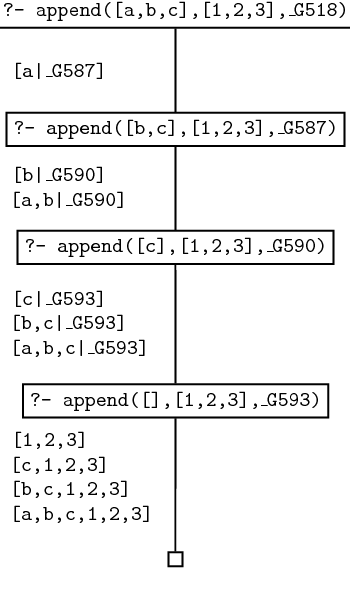
\includegraphics[scale = 0.5]{PrologAppendWorking.png}
\caption{Trace for append \cite{webiste:learnprolognowappend}}
\label{fig:Trace for append}
\end{figure}



\begin{figure}
  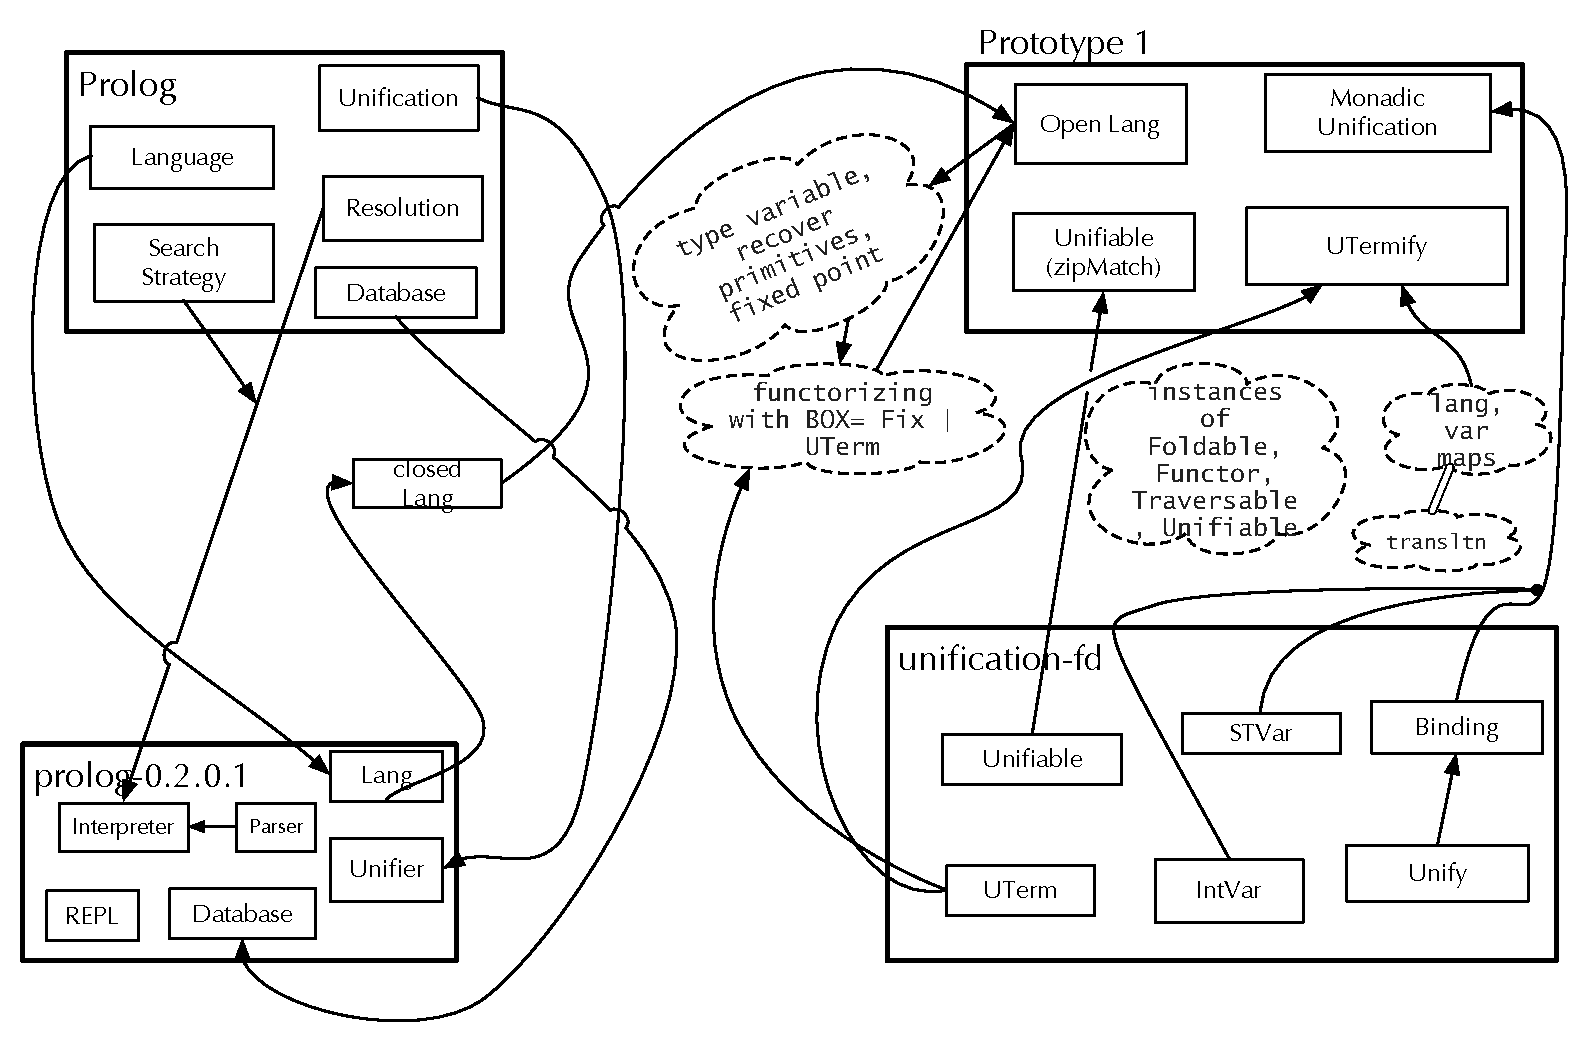
\includegraphics[width=1\textwidth]{Prototype-1.pdf}
  \caption{Architecture of Prototype 1}
  \label{fig:proto1-arch}
\end{figure}

\section{What we do in this Prototype}
This prototype throws light on the process of tackling the issues involved in creating
a data type to replicate the target language type system while conforming to the host language restrictions and also utilizing the
benefits.\endnote{
  \david{simplify}
}


We have a \progLang{Prolog}-like language in \progLang{Haskell} defined via \haskellConstruct{data}. The language defined is recursive in nature. We convert 
it into a non-recursive data type. Basically we do unification monadically.

\section{Creating a data type}

To start we need to define a abstract syntax for the \progLang{Prolog}-like language.
But there is a conflict between the type systems as we shall discuss.


\endnote{
  \david{move to related concepts Start}
}

A type system consists of a set of rules to define a ``type'' to different constructs in a
programming language such as variables, functions and so on.
A static type system requires types to be attached to the programming constructs before hand which results in
finding errors at compile time and thus increase the reliability of the program.
On the other hand the dynamic type system passes through code which would not have worked in former
environment; it comes off as less rigid.


The advantages of static typing \cite{meijer2004static} are :
\begin{itemize}
\item earlier detection of errors,
\item better documentation in terms of type signatures,
\item more opportunities for compiler optimizations,
\item increased run-time efficiency, and
\item better developer tools;
\end{itemize}

whereas for dynamic typing the advantages are:
\begin{itemize}
\item less rigidity,
\item suitability, and
\item re-usability.
\end{itemize}

\endnote{
  \david{move to related concepts end}
}

Since \progLang{Haskell} is statically typed we need to define a ``typed'' language which
has a number of constructs representing different terms in \progLang{Prolog}, such as complex structures
(for example predicates, clauses etc.), don't cares, cuts, variables and so on.

Consider the language in Listing~\ref{tab:closed-terms}, which has been adopted from
\cite{prolog-lib}.

\begin{code-list}
\begin{minted}[linenos]{haskell}
  data VariableName = VariableName Int String
  deriving (Eq, Data, Typeable, Ord)
  data Atom         = Atom      !String
                    | Operator  !String
  deriving (Eq, Ord, Data, Typeable)
  data Term = Struct Atom [Term]
            | Var VariableName
            | Wildcard
            | Cut Int
  deriving (Eq, Data, Typeable)
  data Clause = Clause { lhs :: Term, rhs_ :: [Goal] }
              | ClauseFn { lhs :: Term, fn :: [Term] -> [Goal] }
  deriving (Data, Typeable)
  type Program = [Sentence]
  type Body    = [Goal]
  data Sentence = Query   Body
                | Command Body
                | C Clause
  deriving (Data, Typeable)
\end{minted}
  \caption{A classic recursive grammar}
  \label{tab:closed-terms}
\end{code-list}

Even though \textit{Term} has a number of constructors the resulting construct has a single type.
Hence, a binary function would have type
\par
\begin{minted}{haskell}
foo :: Term -> Term -> Term
\end{minted}

Listing~\ref{tab:closed-terms} is a classic example of using a recursive data type to define the
abstract syntax of a language.
One of the issues with the datatype in Listing~\ref{tab:closed-terms} is that it is not possible to distinguish the structure of the data from
the data type itself \cite{sheard2004two}.
Moreover, the primitives of the language (see \cite{website:understandingalgebrasfpcomplete})\endnote{%
  is this ok?
}
are not accessible, as the language can have expressions of only one
type, ``\haskellConstruct{Term}''.

\begin{comment}
The solution  would be to add a type constructor split the data type into two levels, a single recursive
data type is replaced by two related data types.
\end{comment}
Consider the code in Listing~\ref{tab:non-recurse}
\begin{code-list}
  \begin{minted}[gobble=3,linenos]{haskell}
    data FlatTerm a = Struct Atom [a]
                    | Var VariableName
                    | Wildcard
                    | Cut Int
               deriving (Show, Eq, Ord)
  \end{minted}
  \caption{A flattened (non-recursive) grammar}
  \label{tab:non-recurse}
\end{code-list}

One result of coding as in Listing~\ref{tab:non-recurse} rather than as in
  Listing~\ref{tab:closed-terms} (lines 6--9)
  is that the non-recursive type
\texttt{FlatTerm} is modular and generic as the structure
\haskellConstruct{FlatTerm}
is separate
from its
type which is ``\unknownLabel{\textit{a}}''\eref{text-kind}.
The above language can be of any type \textit{a}.
A more accurate way of saying it would be that \textit{a} can be a \textit{kind} in
\progLang{Haskell}.\endnote{%
  Why do we explain \textit{kinds}?
  Is this in preparation for \texttt{\bfseries Functor}?
  \mehul{Well Int, String etc etc are kinds in haskell so a FlatTerm int where int is *}
}

In type theory, a kind is the type of a type constructor or, less commonly, the type of a higher-order type operator. A kind system is
essentially a simply typed lambda calculus 'one level up,' endowed with a primitive type, denoted * and called 'type,' which is the kind of
any (monomorphic) data type for example \cite{website:kindhaskellwiki},

\begin{minted}[linenos,frame=lines]{haskell}
Int :: *
Maybe :: * -> *
Maybe Bool :: *
a -> a :: *
[] :: * -> *
(->) :: * -> * -> *
\end{minted}

Simply speaking we can have something like
\mint{haskell}|FlatTerm Bool|
and a generic function like,
\mint{haskell}|function :: (a -> b) -> FlatTerm a -> FlatTerm b|
\begin{comment}
  I think this is more to say all terms in the language can be (FlatTerm a) and not
  (FlatTerm (FlatTerm (FlatTerm ....)))
\end{comment}
One problem remains: how does one represent deep expressions
of the above language, 
for example something of the form,
\mint{haskell}|FlatTerm(FlatTerm (FlatTerm (FlatTerm (....... (a)))))|
and how to represent it generically to perform operations on it, since
\begin{minted}[linenos]{haskell}
(FlatTerm a) != (FlatTerm (FlatTerm a))
\end{minted}
%
because with our original grammar all the expression that could be defined would be represented by a single entity
\haskellConstruct{Term} no matter how infinitely deep they were.

The approach to tackling this problem is to find the ``fixed-point''.
After infinitely many iterations we should get to a fixed point where further iterations make no
difference.
It means that applying one more \haskellConstruct{FlatTerm} would not change anything --\textsuperscript{,}\endnote{%
  An en-dash is not appropriate here.
}
a \textcolor{red}{fix}\endnote{%
  Spelling!
}
point does not move under \haskellConstruct{FlatTerm}.

\progLang{Haskell} provides it in two forms,\endnote{%
  \david{Why do you need to discuss value fixed points (\textit{i.e.,} \texttt{\bfseries fix})?  Do you need them?} 

  \mehul{Well not really but since we are talking about fixed point in general}

  \david{Get rid of it.  Put in a marker if you want.  If we really need it, we can drag it from the git repository.}
}
\begin{enumerate}

\item The \markWord{fix} function in the \texttt{Control.Monad.Fix} module allows for the definition of recursive functions in \progLang{Haskell}. Consider the following scenario,

\mint{haskell}|fix :: (a -> a) -> a|

The above function results in an infinite application stream,
\mint{haskell}|f s : f (f (f (... )))|

A fixed point of a function \markWord{f} is a value a such that \markWord{f a} \Verb!==! \markWord{a}.
This is where the name of fix comes from: it finds the least-defined fixed
point of a function.

\item In type constructor form,
\mint{haskell}|newtype Fix f = f (Fix f)|
which we apply to our abstract syntax.

\end{enumerate}


The resulting language is of the form,
\begin{minted}[linenos]{haskell}
data Prolog = P (Fix FlatTerm) deriving (Show,Eq,Ord)
\end{minted}
%
simply speaking all the expressions resulting from \haskellConstruct{FlatTerm} can be represented  by the type signature \haskellConstruct{Fix FlatTerm}.

A sample function working with such expressions would be of the form,
\mint{haskell}|func :: Fix FlatTerm -> Fix FlatTerm|


Generically speaking, the language can be expanded for additional functionality without changing or modifying the base structure. Consider
the scenario where the language needs to accommodate additional type of terms,

\begin{enumerate}
\item Manually modifying the structure of the language, as shown in Listing~\ref{tab:man-enhan-gram}
  \begin{code-list}
    \begin{minted}[linenos,gobble=5]{haskell}
      type Atom            = String

      data VariableName    = VariableName Int String
      deriving (Eq, Data, Typeable, Ord)

      data Term  = Struct Atom [Term]
                 | Var VariableName
                 | Wildcard
                 | Cut Int
                 | New_Constructor_1 .........
                 | New_Constructor_2 .........
        deriving (Eq, Data, Typeable)
    \end{minted}
    \caption{A manually enhanced recursive grammar}
    \label{tab:man-enhan-gram}
  \end{code-list}

This would then trigger a ripple effect throughout the architecture because accommodations need to be made for the new functionality.

\item The other option would be to \textit{functorize} language like we did by adding a type variable which can be used to plug something that provides the functionality into the language.
Consider the following example,

\begin{minted}[linenos]{haskell}
data Box f = Abox | T f (Box f) deriving (.........)
\end{minted}

then something like,
\begin{minted}[linenos]{haskell}
T (Struct 'atom' [Abox, T (Cut 0)])
\end{minted}
\end{enumerate}
is possible. Since we needed the fixed point of the language we used \textit{Fix} but generically one could add multiple custom
functionality.

%%====================================================================%%
%% -- begin code inserted by David                                 -- %%
%---------------------------------------------------------------------%%
\begin{center}
  \textcolor{blue}{\rule{0.95\textwidth}{0.2em}}\\[-1ex]
  text from David
\end{center}
Why not continue the example that you started in Figure~\ref{tab:man-enhan-gram}?
That is use code something like that in Figure~\ref{tab:garfunkle}, and show how
\Verb!Extended FlatTerm! is isomorphic to \Verb!Term! from Figure~\ref{tab:man-enhan-gram}?

\begin{code-list}[h]
  \begin{minted}[linenos,gobble=2]{haskell}
    data Extended f  = New_Constructor_1 ...
                     | New_Constructor_2 ....
                     | Base (f (Extended f))
  \end{minted}
  \caption{garfunkle}
  \label{tab:garfunkle}
\end{code-list}
\vspace*{-1.5\baselineskip}
\begin{center}
  end text from David\\[-3ex]
  \textcolor{blue}{\rule{0.95\textwidth}{1pt}}
\end{center}
%---------------------------------------------------------------------%%
%% -- end code inserted by David                                   -- %%
%%====================================================================%%

\Figure~\ref{fig:manual_extension} \Figure~\ref{fig:automatic_extension}

\begin{figure}
  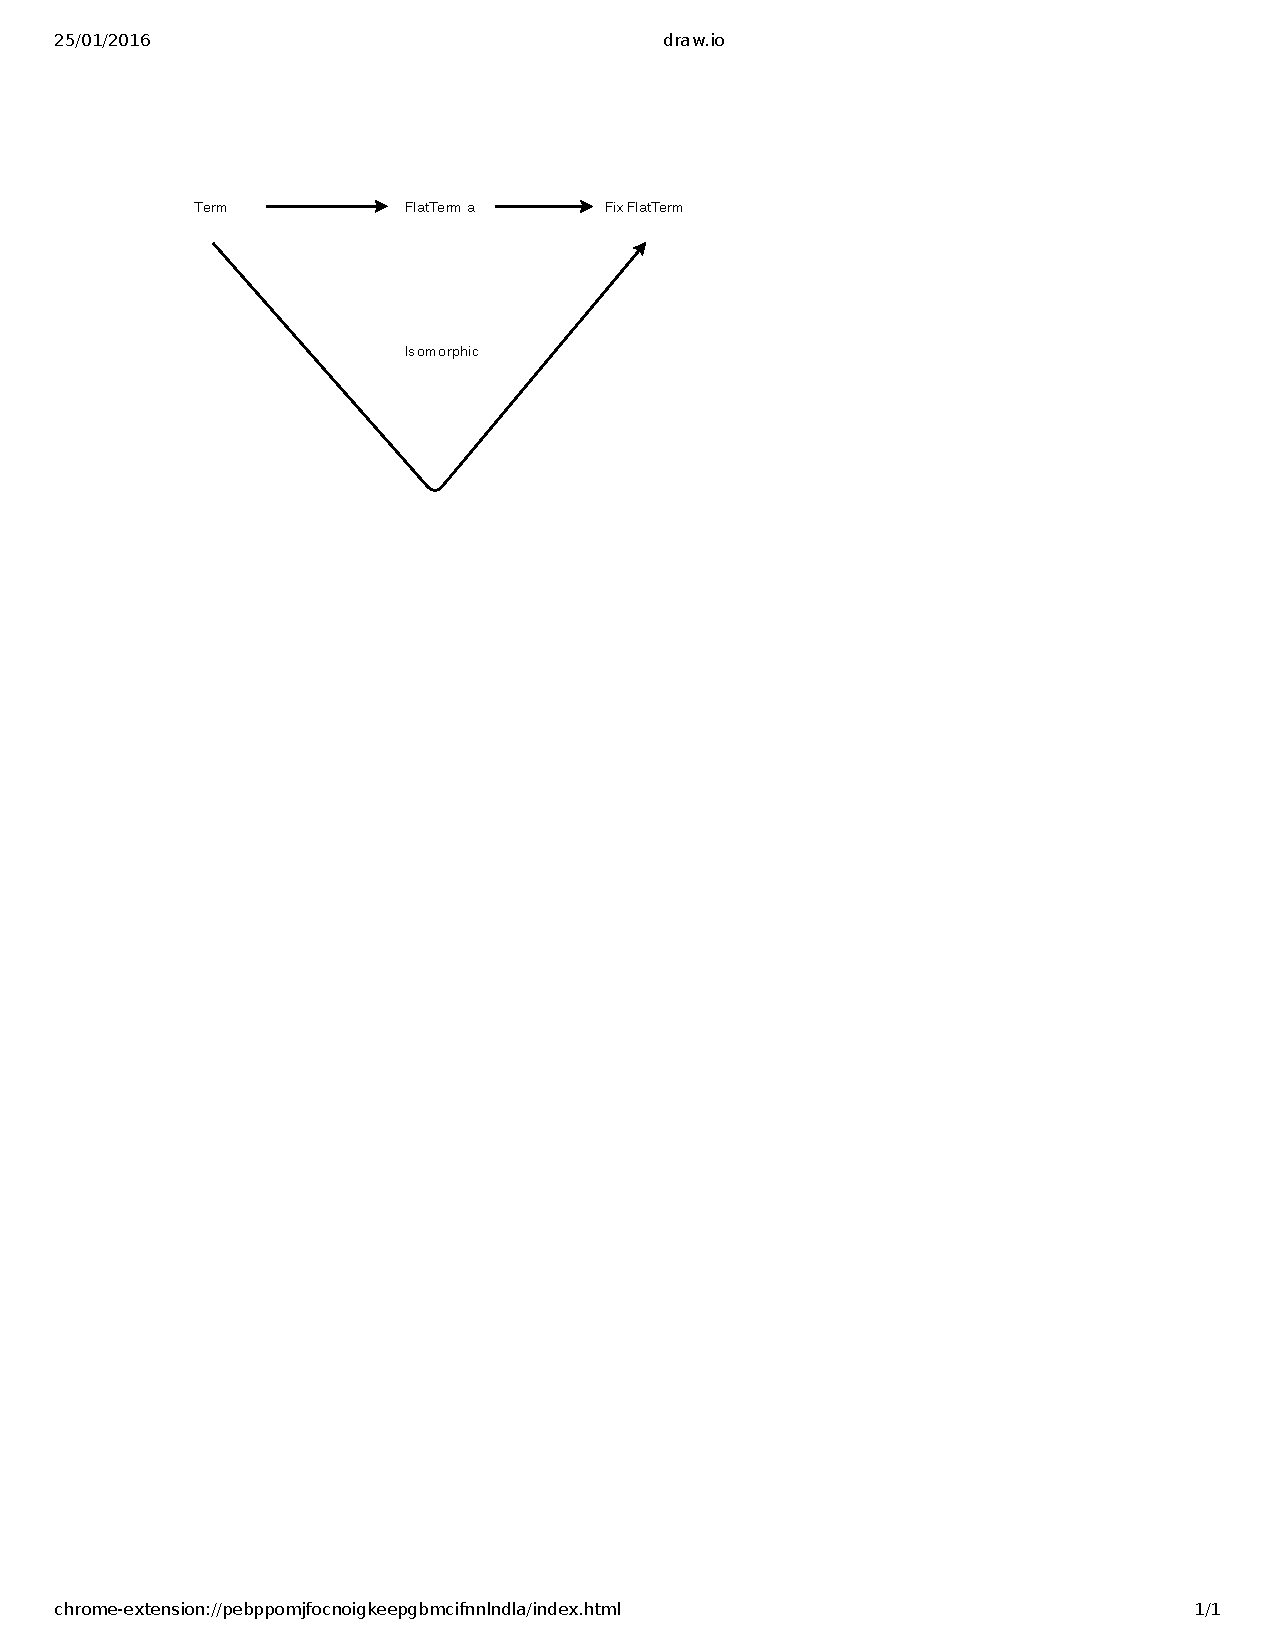
\includegraphics[width=1\textwidth]{extended_data_type_1.pdf}
  \caption{Manually Extension of data type}
  \label{fig:manual-extension}
\end{figure}

\begin{figure}
  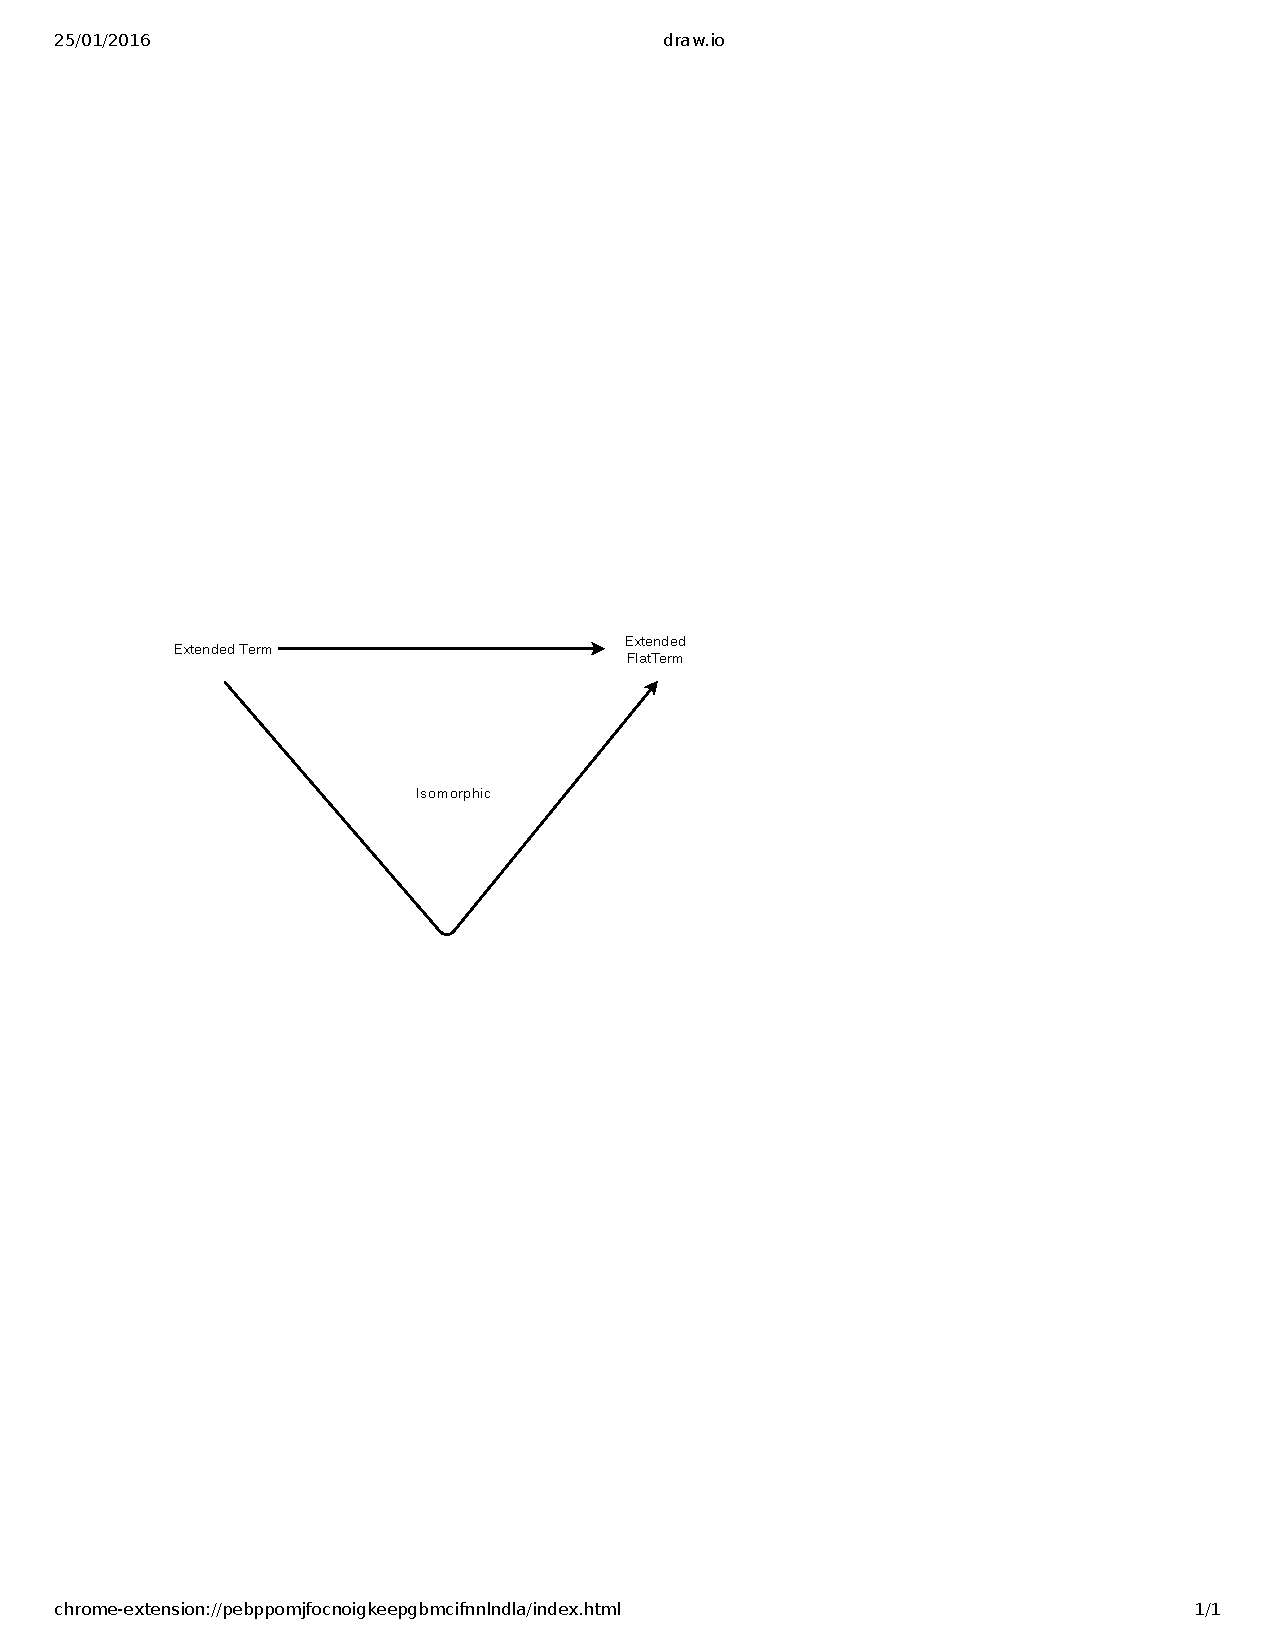
\includegraphics[width=1\textwidth]{extended_data_type_2.pdf}
  \caption{Automatic Extension of data type}
  \label{fig:automatic-extension}
\end{figure}

\section{Making the language compatible with \protect\codeLibrary{unification-fd}}\label{sec:making-lang-comp}

\david{Check the Section~\ref{sec:making-lang-comp} title change above.}

Our language is now opened up and ready for expansion, but it still needs to conform to the requirements of the
\codeLibrary{unifiication-fd} library (\cite{unification-fd-lib}), so that the generic unification algorithm upon
customization works with it.\endnote{%
  This sentence can be simplified, I think.}

  The library provides functionality for first-order structural unification over general structure types along with
  mutable variable bindings.

In this section we discuss
\begin{enumerate}
\item Functor hierarchy.

\item Required instances the language must have.

\item Mutable variables.

\item Variable bindings.

\item Monadic unification.

\item Replicating \progLang{Prolog} unification in \progLang{Haskell}
\end{enumerate}

Classes in \progLang{Haskell} are like containers with certain properties which can be thought of as functions. When a data type creates an
instance of a class the function(s) can be applied to each element / primitive in the data type.


The data here is the \progLang{Prolog} abstract syntax and the containers are
\Verb!Functor!, \Verb!Foldable!, \Verb!Traversable!, \Verb!Applicative!
  and
\Verb!Monad!.\endnote{%
  Removed the \macroName{clearpage}.
}

Figure~\ref{fig:Functor Hierarchy} shows the relation between the different classes.

\begin{figure}[th]
\centering
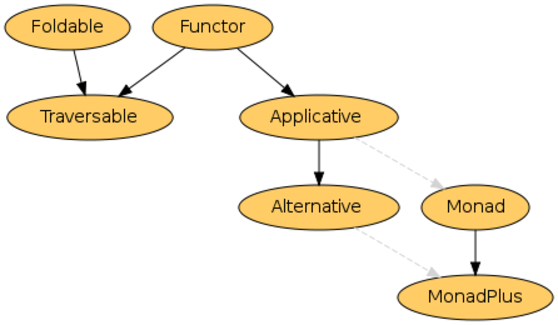
\includegraphics[scale = 0.7]{FunctorHierarchy.png}
\caption{Functor Hierarchy \cite{website:foldablenadtraversable}}
\label{fig:Functor Hierarchy}
\end{figure}

The \Verb!Functor! and \Verb!Foldable! instances providing functions for applying map-reduce\endnote{
It allows reduce whilst preserving the shape of the structure.
Lastly, the \markWord{Applicative} instance is an intermediate between a functor and a monad.

We create the necessary instances\endnote{%
  I am deeply suspicious of the instance for \texttt{Applicative} given.

  \mehul{I agree, I think I just created one for the purpose of the diagram.}
}
as shown in Listing~\ref{tab:flat-term-class-inst}.
\begin{code-list}
  \begin{singlespace}
    \inputminted[linenos,gobble=4]{haskell}{haskell-proto1-class-flat.hs}
  \end{singlespace}
  \caption{FlatTerm class instances}
  \label{tab:flat-term-class-inst}
\end{code-list}

The above lay the foundation to work with the library.
Coming back to the library, the language must have the \Verb!Unifiable! instance.
This works in tandem with the \Verb!UTerm! data type.
The \Verb!UTerm! data type captures the recursive structure of logic terms, i.e., given
some functor \(t\) which describes the 
constructors of our logic terms, and some type \(v\) which describes our logic variables, the type
\Verb!UTerm! \(t\) \(v\) is the
type of logic terms: trees with multiple layers of \(t\) structure and leaves of type \(v\).
The \Verb!Unifiable! class gives one step of the unification process.
Just as we only need to specify one level of the ADT (i.e., \Verb!T!) and then we can use the library's \Verb!UTerm! to generate
the recursive ADT, so too we only need to specify one level of the unification (i.e., \Verb!zipMatch!) and then we can use
the library's operators to perform the recursive unification.
This is shown in Figure~\ref{tab:zipMatch}.
\begin{code-list}
  \begin{singlespace}
    \inputminted[linenos]{haskell}{haskell-proto1-zip-flat.hs}
  \end{singlespace}
  \vspace*{-0.5\baselineskip}
  \caption{\protect\markWord{FlatTerm} instance of \protect\markWord{zipMatch}}
  \label{tab:zipMatch}
\end{code-list}

\paragraph{Logic Variables}
Unification involves side effects of binding logic variables to terms. To allow and keep track of these effects we use the binding monad
which provides facilities to generate fresh logic variables and perform look ups on dictionaries. By default two logic variable
implementations exist,\endnote{%
  In this immediate region, I (dgc) removed text inserted by a failed push or pull merge.
  Check to see that it is correct, or reverse commit \texttt{95804e3\dots}.
}

\begin{enumerate}
\item The \markWord{IntVar} implementation uses \markWord{Int} as the names of variables, and uses an
  \markWord{IntMap} to keep track of the environment. 

\item The \markWord{STVar} implementation uses \markWord{STRef}s, so we can use actual mutation for binding logic
  variables, rather than keeping an explicit environment around.

\end{enumerate}

\begin{comment}
  The library ships with two implementations of logic variables.
  The \markWord{IntVar} implementation uses \markWord{Int} as the names of variables, and uses an \markWord{IntMap}
  to keep track of the 
  environment.
  The \markWord{STVar} implementation uses \markWord{STRefs}, so we can use actual mutation for binding logic variables, rather than
  keeping an explicit environment around.
  This implementation uses \markWord{STVars}.

  Performing unification has the side effect of binding logic variables to terms.
  Thus, we'll want to use a monad in order to keep track of these effects.
  The \markWord{BindingMonad} type class provides the definition of what we need from our ambient monad.
  In particular, we need to be able to generate fresh logic variables, to bind logic variables, and to lookup what
  our logic variables are bound to.
  The library provides the necessary instances for both \markWord{IntVar} and \markWord{STVar}.

  You can provide your own implementations of \markWord{Variable} and \markWord{BindingMonad}.
\end{comment}

\textbf{Some stuff about Meta syntactic variables can be put in here}

This implementation uses \markWord{STVars}
but a custom implementation can be used inside the \markWord{BindingMonad}.
For our language expressions to be unifiable we must deal with the variables in the expressions being compared.
For that we extract the variables and then convert them into a dictionary consisting of a free variable for each
language variable as shown in Figure~\ref{tab:varsToDictM}.

\begin{code-list}
  \begin{minted}[linenos,gobble=2]{haskell}
  variableExtractor :: Fix FlatTerm -> [Fix FlatTerm]
  variableExtractor (Fix x) = case x of
     (Struct _ xs) ->   Prelude.concat $ Prelude.map variableExtractor xs
     (Var v)      ->   [Fix $ Var v]
     _         ->   []

  variableNameExtractor :: Fix FlatTerm -> [VariableName]
  variableNameExtractor (Fix x) = case x of
     (Struct _ xs)   -> Prelude.concat $ Prelude.map variableNameExtractor xs
     (Var v)         -> [v]
     _             -> []

  variableSet :: [Fix FlatTerm] -> S.Set (Fix FlatTerm)
  variableSet a = S.fromList a

  variableNameSet :: [VariableName] -> S.Set (VariableName)
  variableNameSet a = S.fromList a

  varsToDictM :: (Ord a, Unifiable t) =>
      S.Set a -> ST.STBinding s (Map a (ST.STVar s t))
  varsToDictM set = foldrM addElt Map.empty set where
    addElt sv dict = do
      iv <- freeVar
      return $! Map.insert sv iv dict
  \end{minted}
  \vspace*{-1.0\baselineskip}
  \caption{Creating a variable dictionary}
  \label{tab:varsToDictM}
\end{code-list}
A language to \markWord{STVar} dictionary is only one part of the unification procedure, the terms themselves should be made
compatible for the in built unify procedure to perform look ups for the variables in them.
The dictionary along with the fixed point version flattened of the term, as shown in Figure~\ref{tab:to-UTerm}.
%
\begin{code-list}
  \begin{minted}[linenos,gobble=2]{haskell}
  uTermify
    :: Map VariableName (ST.STVar s (FlatTerm))
    -> UTerm FlatTerm (ST.STVar s (FlatTerm))
    -> UTerm FlatTerm (ST.STVar s (FlatTerm))
  uTermify varMap ux = case ux of
    UT.UVar _                -> ux
    UT.UTerm (Var v)        -> maybe (error "bad map") UT.UVar $
                                 Map.lookup v varMap
    -- UT.UTerm t            -> UT.UTerm $! fmap (uTermify varMap)
    UT.UTerm (Struct a xs)   -> UT.UTerm $ Struct a $!
                                         fmap (uTermify varMap) xs
    UT.UTerm (Wildcard)      -> UT.UTerm Wildcard
    UT.UTerm (Cut i)         -> UT.UTerm (Cut i)

  translateToUTerm ::
      Fix FlatTerm -> ST.STBinding s
              (UT.UTerm (FlatTerm) (ST.STVar s (FlatTerm)),
               Map VariableName (ST.STVar s (FlatTerm)))
  translateToUTerm e1Term = do
    let vs = variableNameSet $ variableNameExtractor e1Term
    varMap <- varsToDictM vs
    let t2 = uTermify varMap . unfreeze $ e1Term
    return (t2,varMap)
  \end{minted}
  \caption{Conversion to UTerm}
  \label{tab:to-UTerm}
\end{code-list}
%
and for later use to convert them back, as shown in Figure~\ref{tab:from-UTerm}.
%
\begin{code-list}
  \begin{minted}[linenos,gobble=2]{haskell}
  vTermify :: Map Int VariableName ->
              UT.UTerm (FlatTerm) (ST.STVar s (FlatTerm)) ->
              UT.UTerm (FlatTerm) (ST.STVar s (FlatTerm))
  vTermify dict t1 = case t1 of
    UT.UVar x  -> maybe (error "logic") (UT.UTerm . Var) $
                           Map.lookup (UT.getVarID x) dict
    UT.UTerm r ->
      case r of
        Var iv   -> t1
        _         -> UT.UTerm . fmap (vTermify dict) $ r

  translateFromUTerm ::
      Map VariableName (ST.STVar s (FlatTerm)) ->
      UT.UTerm (FlatTerm) (ST.STVar s (FlatTerm)) -> Prolog
  translateFromUTerm dict uTerm =
    P .  maybe (error "Logic") id . freeze . vTermify varIdDict $ uTerm where
      rot3 f a k v = f k v a
      inserter k v = Map.insert (UT.getVarID v) k
      forKV dict initial fn = Map.foldlWithKey' (rot3 fn) initial dict
      varIdDict = forKV dict Map.empty inserter
  \end{minted}
  \caption{Conversion from UTerm}
  \label{tab:from-UTerm}
\end{code-list}

\clearpage
The variable dictionaries and \markWord{UTerm}ified language expressions are unified in the binding monad as shown
in Figure~\ref{tab:unification} and Figure~\ref{tab:unif-driver}.
%
\begin{code-list}
\begin{minted}[linenos]{haskell}
  monadicUnification ::
  (BindingMonad FlatTerm (STVar s FlatTerm) (ST.STBinding s))
  => (forall s. ((Fix FlatTerm) -> (Fix FlatTerm)
  ->  ErrorT (UT.UFailure (FlatTerm) (ST.STVar s (FlatTerm)))
             (ST.STBinding s) (UT.UTerm (FlatTerm) (ST.STVar s (FlatTerm)),
                               Map VariableName (ST.STVar s (FlatTerm)))))
monadicUnification t1 t2 = do
--  let
--    t1f = termFlattener t1
--    t2f = termFlattener t2
  (x1,d1) <- lift . translateToUTerm $ t1
  (x2,d2) <- lift . translateToUTerm $ t2
  x3 <- U.unify x1 x2
  --get state from somehwere, state -> dict
  return $! (x3, d1 `Map.union` d2)
\end{minted}
  \vspace*{-1.0\baselineskip}
  \caption{Unification code}
  \label{tab:unification}

\begin{minted}[linenos]{haskell}
goUnify ::
  (forall s. (BindingMonad FlatTerm (STVar s FlatTerm) (ST.STBinding s))
  =>
      (ErrorT
          (UT.UFailure FlatTerm (ST.STVar s FlatTerm))
          (ST.STBinding s)
          (UT.UTerm FlatTerm (ST.STVar s FlatTerm),
             Map VariableName (ST.STVar s FlatTerm)))
     )
  -> [(VariableName, Prolog)]
goUnify test = ST.runSTBinding $ do
  answer <- runErrorT $ test --ERROR
  case answer of
    (Left _)            -> return []
    (Right (_, dict))   -> f1 dict
\end{minted}
  \vspace*{-1.0\baselineskip}
  \caption{Driver code}
  \label{tab:unif-driver}
\end{code-list}


The final reconversion to return a list of substitutions,
  called \texttt{f1} in Figure~\ref{tab:unif-driver}, is shown in
  Figure~\ref{tab:vars-extract}.
\begin{code-list}
  \begin{minted}[linenos,gobble=2]{haskell}
  f1 ::
    (BindingMonad FlatTerm (STVar s FlatTerm) (ST.STBinding s))
    => (forall s. Map VariableName (STVar s FlatTerm)
        -> (ST.STBinding s [(VariableName, Prolog)])
       )
  f1 dict = do
    let ld1 = Map.toList dict
    ld2 <- Control.Monad.Error.sequence
           [ v1 | (k,v) <- ld1, let v1 = UT.lookupVar v]
    let ld3 = [ (k,v) | ((k,_),Just v) <- ld1 `zip` ld2]
        ld4 = [ (k,v) | (k,v2) <- ld3,
                let v = translateFromUTerm dict v2 ]
    return ld4
  \end{minted}
  \vspace*{-1.0\baselineskip}
  \caption{Variable substitution list extraction}
  \label{tab:vars-extract}
\end{code-list}

\section{Chapter Recapitulation}

\ifMain
\begin{scope}
  \nolinenumbers
  \enotesize
  \par
  \begin{singlespace}
  \setlength{\parskip}{12pt plus 2pt minus 1pt}
  \theendnotes
  \par
  \end{singlespace}
\end{scope}
\unbcbibliography{bibliography}
\fi

\end{document}
